\chapter{Мета-моделирование}

К последнее десятилетие широкое распространение получили \term{объектно-ориентированные модели программного обеспечения} и \term{мета-моделирование} (Meta-Modeling, \cite{MetaModeling}). Этот подход используется для проектирования, документирования и автоматического построения ПО. Он получил признание благодаря UML, унифицированному языку моделирования (Unified Modeling Language, \cite{UML}) и MDA, архитектуре, управляемой моделями (Model-Driven Architecture, \cite{MDA}).
Позднее возникли и другие языки и технологии, опирающиеся на те же принципы.

В данном разделе мы приводим основные определения и примеры, необходимые для понимания концепции мета-моделирования. 

\section{Модели}

Одним из центральных понятий в данной области является ``объектно-ориентированная модель''.  Также говорят ``модель предметной области'' или просто ``модель''. Под моделью понимается структурированное описание некоторой сущности реального мира (например, программной или аппаратной системы, инфраструктуры предприятия и т.д.). С формальной точки зрения модель представляет собой граф, вершинами в котором являются типизированные объекты, обладающие типизированными атрибутами \cite{KM3}. Естественным визуальным представлением моделей являются \term{диаграммы}; в качестве примера рассмотрим простую диаграмму модели зависимостей между компонентами ПО (\figref{DiagramExample}).

\begin{figure}[htbp]
// Диаграмма: модель билда с зависимостями
\caption{Модель зависимостей между компонентами ПО}\label{DiagramExample}
\end{figure}

Вершины графа на \figref{DiagramExample} соответствуют компонентам, а ребра --- зависимостям. Каждое ребро направлено от зависимой компоненты (\term{клиента}) к компоненте, от которой она зависит (к \term{серверу}). Таким образом, данная модель состоит из трех объектов, ссылающихся друг на друга. Аналогично объектно-ориентированным языкам программирования \cite{JLS}, каждый объект имеет тип, определяемый его классом. В данном случае все три объекта относятся к одному классу \code{Component} (см. \figref{ComponentClass}). 

\begin{figure}[htbp]
// Код, UML-диаграмма и диаграмма объектов для класса Component
class Component {
	attr name : String;
	ref dependsOn : Component[*];
}
\caption{Мета-модель для компонент}\label{ComponentClass}
\end{figure}

На \figref{ComponentClass} (a) приведен псевдокод объявления класса Component. Данный класс декларирует \term{атрибут} \code{name} \term{примитивного типа} \code{String}, значение которого на диаграмме отображается внутри вершины, и \term{ссылку} \code{dependsOn} типа \code{Component}, значения которой на диаграмме отображаются в виде ребер между объектами типа \code{Component}. Поскольку одна компонента может зависеть от нескольких других компонент, ссылка \code{dependsOn} является \term{множественной}, что определяется аннотацией в квадратных скобках (``*'' соответствует кратности (multiplicity) ``ноль или более'').

Во многих объектно-ориентированных языках программирования (\tool{Java}, \tool{C\#}, \tool{SmallTalk} \cite{SmallTalk}) классы являются также и объектами. В нашем случае мы можем описать класс \code{Component} как модель. Как видно из \figref{ComponentClass} (b), эта модель состоит из следующих объектов: 
\begin{enumerate}
\item самого класса \code{Component};
\item атрибута \code{name};
\item ссылки \code{dependsOn};
\item типа \code{String}.
\end{enumerate}
Все объекты имеют имена, а ссылка \code{dependsOn} -- еще и кратность.
Ребра на диаграмме подписаны в соответствии со связями, которые они отображают: класс владеет атрибутами и ссылками, атрибуты и ссылки имеют типы. 

Одну и ту же модель можно изображать с помощью диаграмм по-разному, так на \figref{ComponentClass} (c) показана та же самая модель для класса Component, отображенная в виде стандартной диаграммы классов языка UML \cite{UML}. Как видно из рисунка, эта диаграмма является более компактной за счет того, что атрибут отображаются внутри вершины, соответствующей классу, который ими владеет, а ссылки --- в виде ребер, направленных от класса, который владеет ссылкой, к классу, являющемуся типом ссылки (в UML ссылки моделируются с помощью \term{ассоциаций}, обладающих гораздо более выразительной семантикой, и в частности, позволяющих выразить отношения произвольной арности \cite{???}). Этот пример является очень полезным, поскольку позволяет увидеть, что объект, имеющийся в модели (ссылка), может быть изображен на диаграмме в виде ребра.

\section{Мета-модели и иерархия мета-уровней}

Модель, изображенная на \figref{ComponentClass} описывает типы элементов модели, изображенной на \figref{DiagramExample}, то есть является для нее \term{мета-моделью}. Каждый элемент на диаграмме \figref{ComponentClass} имеет соответствующий элемент в мета-модели (\term{мета-элемент}), и называется его \term{экземпляром}. Отношение ``экземпляр-мета-элемент'' проиллюстрировано на \figref{ConformsToRelation}.

\begin{figure}[htbp]
\caption{Отношение ``экземпляр-мета-элемент''}\label{ConformsToRelation}
\end{figure}

Поскольку в любой модели все объекты типизированы, каждая модель имеет мета-модель  (то есть любая модель является экземпляром некоторой мета-модели). Говорят об ``иерархии мета-уровней'', которые схематически изображены на \figref{ConformsToRelation}  и помечены как $M^1$, $M^2$, $M^3$\ldots Модели уровня $M^{i+1}$ являются мета-моделями для моделей уровня $M^i$. В принципе, иерархия мета-уровней может быть сколь угодно высокой или даже бесконечной, но для практических целей обычно используется иерархия из трех уровней. Это достигается за счет эффекта ``раскрутки'' (bootstrapping, см. \cite{Wirth}): на уровне $M^3$ помещается ровно одна мета-модель, которая типизирует сама себя. Такая модель называется \term{мета-мета-моделью}, именно мета-мета-модели обычно составляют основу модельно-ориентированных инструментов разработки и стандартов, таких как MOF \cite{MOF}, KM3 \cite{KM3}, VPM \cite{VPM} или \tool{Ecore} \cite{EMF}. Большинство используемых на практике мета-мета-моделей эквивалентны по выразительности, то есть существуют автоматизированные средства преобразования между их экземплярами (см. напр. \cite{KM3}). Здесь и далее мы будем использовать мета-мета-модель \tool{Ecore}, которая лежит в основе библиотеки EMF (Eclipse Modeling Framework, \cite{EMF}) и хорошо зарекомендовала себя в качестве платформа для разработки приложений с использованием моделей.

\section{Мета-мета-модель \tool{Ecore}}

\begin{figure}[htbp]
\centering
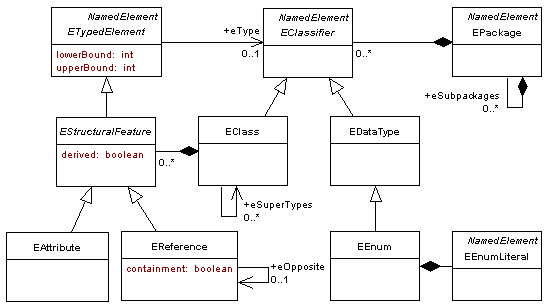
\includegraphics[width=\textwidth]{ecore.png}
\caption{Мета-мета-модель \tool{Ecore}}\label{Ecore}
\end{figure}

На \figref{Ecore} изображена диаграмма мета-мета-модели \tool{Ecore}. Согласно объектно-ориентированной парадигме, центральным понятием в \tool{Ecore} является класс. Экземпляры \tool{Ecore} (то есть мета-модели) представляют собой наборы классов, организованные в пакеты и связанные отношением ``общее-частное'', аналогичным наследованию в объектно-ориентированных языках программирования \cite{OOAD}. На \figref{ComponentClassEcore} показано, как элементы мета-модели, описывающей модели зависимостей между компонентами (такие как \figref{DiagramExample}) связаны с соответствующими мета-элементами в \tool{Ecore}.

//ComponentClassEcore

Следует обратить внимание на то, что \tool{Ecore} сама состоит из классов, что и позволяет ``оборвать'' иерархию мета-уровней, не используя $M^4$ (в действительности, иерархия не обрывается, просто все уровни, начиная с $M^3$ совпадают между собой и содержат только мета-мета-модель, то есть в нашем случае --- \tool{Ecore}).

В этом разделе мы опишем несколько основных концепций, используемых \tool{Ecore} (и другими мета-мета-моделями), которые будут использованы при изложении дальнейшего материала.

\paragraph*{Классы.} Как мы уже отмечали выше, основными элементами мета-моделей, описанных с помощью \tool{Ecore}, являются классы. Каждый класс имеет имя уникальное в пределах пакета, список суперклассов и список структурных элементов, атрибутов и ссылок. Экземпляры классов хранят значения для всех атрибутов и ссылок, объявленных самим классом и всеми его суперклассами (что соответствует наследованию членов классов в объектно-ориентированных языках). Класс может быть помечен как абстрактный. Такой класс не может иметь непосредственных экземпляров, экземпляры могут иметь только его подклассы, не являющиеся абстрактными.

Заметим, что понятие абстрактного класса в \tool{Ecore} является чисто номинальным, никаких технических препятствий к созданию экземпляра класса (таких как, например в \tool{Java} или \tool{C++}) быть не может, поскольку \tool{Ecore} не определяет тела методов. 

\paragraph*{Примитивные типы и перечисления.} Классы --- не единственное средство типизации в \tool{Ecore}, кроме них используются примитивные типы данных (Data Types) и перечисления (Enums). Примитивный тип данных представляет собой именованную сущность, семантика которой либо не фиксируется, либо определяется тем языком программирования, на котором реализовано моделируемое ПО (в случае \tool{Ecore} это \tool{Java}). 

\tool{Ecore} определяет несколько встроенных типов данных, таких как строки, целые и вещественные числа и т. д.

Перечисления --- это типы имеющие конечное множество значений (литералов).

\paragraph*{Структурные элементы классов: атрибуты и ссылки.} Основное отличие классов и примитивных типов данных --- в их назначении. Классы являются типами объектов, из которых состоят модели, а примитивные типы и перечисления --- типами значений атрибутов этих объектов. Таким образом, ссылки, определяемые классами могут иметь в качестве типа только класс, а атрибуты --- только примитивный тип или перечисление.

В остальном ссылки и атрибуты очень похожи. И те, и другие имеют имя и кратность, которая задается как пара чисел, определяющих нижнюю и верхнюю границу для количества значений, хранимых атрибутом или ссылкой. Так, например, ссылка \code{dependsOn} на \figref{DiagramExample} имеет кратность ``от 0 до $\infty$'', что означает, что компонента может зависеть от нуля или более других компонент. Атрибут \code{name} на том же рисунке имеет кратность ``от 1 до 1'', что означает, что каждая компонента должна иметь имя, причем ровно одно.

Как атрибуты, так и ссылки могут быть помечены как ``упорядоченные''. Этот флаг имеет значение для множественных ссылок и атрибутов (верхняя граница кратности которых больше единицы), и означает, что порядок объектов, на которые указывают ссылки (или значений атрибута) важен. Например, в классе \code{Block}, описывающего блок кода в программе и имеющего ссылку \code{statements}, указывающую на последовательность предложений внутри блока, ссылка \code{statements} должна быть упорядоченной, поскольку нам важно знать, в каком порядке выполнять предложения, из которых состоит блок.

\paragraph*{Перекрестные ссылки и агрегация.} Ссылки в \tool{Ecore} подразделяются на два вида: \term{перекрестные} и \term{агрегирующие}. Различие состоит в том, что на один объект не может быть более одной агрегирующей ссылки, то есть объект, имеющий агрегирующую ссылку, ``владеет'' объектом, на который ссылается. Для перекрестных ссылок таких ограничений нет, на любой объект может быть сколько угодно перекрестных ссылок.

Таким образом, если рассматривать модель как граф, ребрами в котором являются ссылки, то любой цикл обязан проходить хотя бы по одной перекрестной ссылке, а агрегирующие ссылки в модели определяют остовный лес \cite{cormen01introduction}.

Явное выделение агрегирующих ссылок позволяет легко представлять модели в древовидной форме, как показано на \figref{ModelTree}.

\begin{figure}[htbp]
\centering
%\includegraphics[width=\textwidth]{model_tree.jpg}
\caption{Представление модели в древовидной форме}\label{ModelTree}
\end{figure}

\paragraph*{Параметризованные типы.} Поскольку \tool{Ecore} развивается на платформе \tool{Java}, с выходом \tool{Java} 5 в мета-мета-модель были добавлены \term{обобщенные типы} (generic types, \cite{GJ}). Любой класс или тип данных может иметь параметры, которые могут служить типами для структурных элементов.

\section{Текстовая нотация для мета-моделей}
//
